\documentclass[UTF8, fontset=windows]{article}
\usepackage{amsmath}
\usepackage[utf8]{inputenc}
\usepackage[T1]{fontenc}
\usepackage{enumitem}
\usepackage[UTF8, nocap]{ctex}
\usepackage{geometry}
\usepackage{listings}
\usepackage{xcolor}
\usepackage{hyperref}
\usepackage{graphicx}
\usepackage{tcolorbox}
\usepackage{tabularx}
\geometry{a4paper, margin=1in}



\title{\textbf{现有大语言模型路径引导策略说明}}
\author{第七组 \\ 
李鹏达 10225101460 \\
张耘彪 10225101437 \\
武泽恺 10225101429
}
\date{2025年3月11日}

\begin{document}
\maketitle

\section*{策略概述}

现有LLM辅助事件生成策略是一种结合了大型语言模型的策略,它可以在应用的GUI 测试中遇到难以通过传统随机策略探索的状态时,利用LLM 生成更有效的输入事件。这种策略特别适用于那些需要深入探索应用状态空间或需要优化测试覆盖率的场景。我们绘制了策略的流程图,如图\ref{fig:llm_strategy}所示。

\begin{figure}[h!]
    \centering
    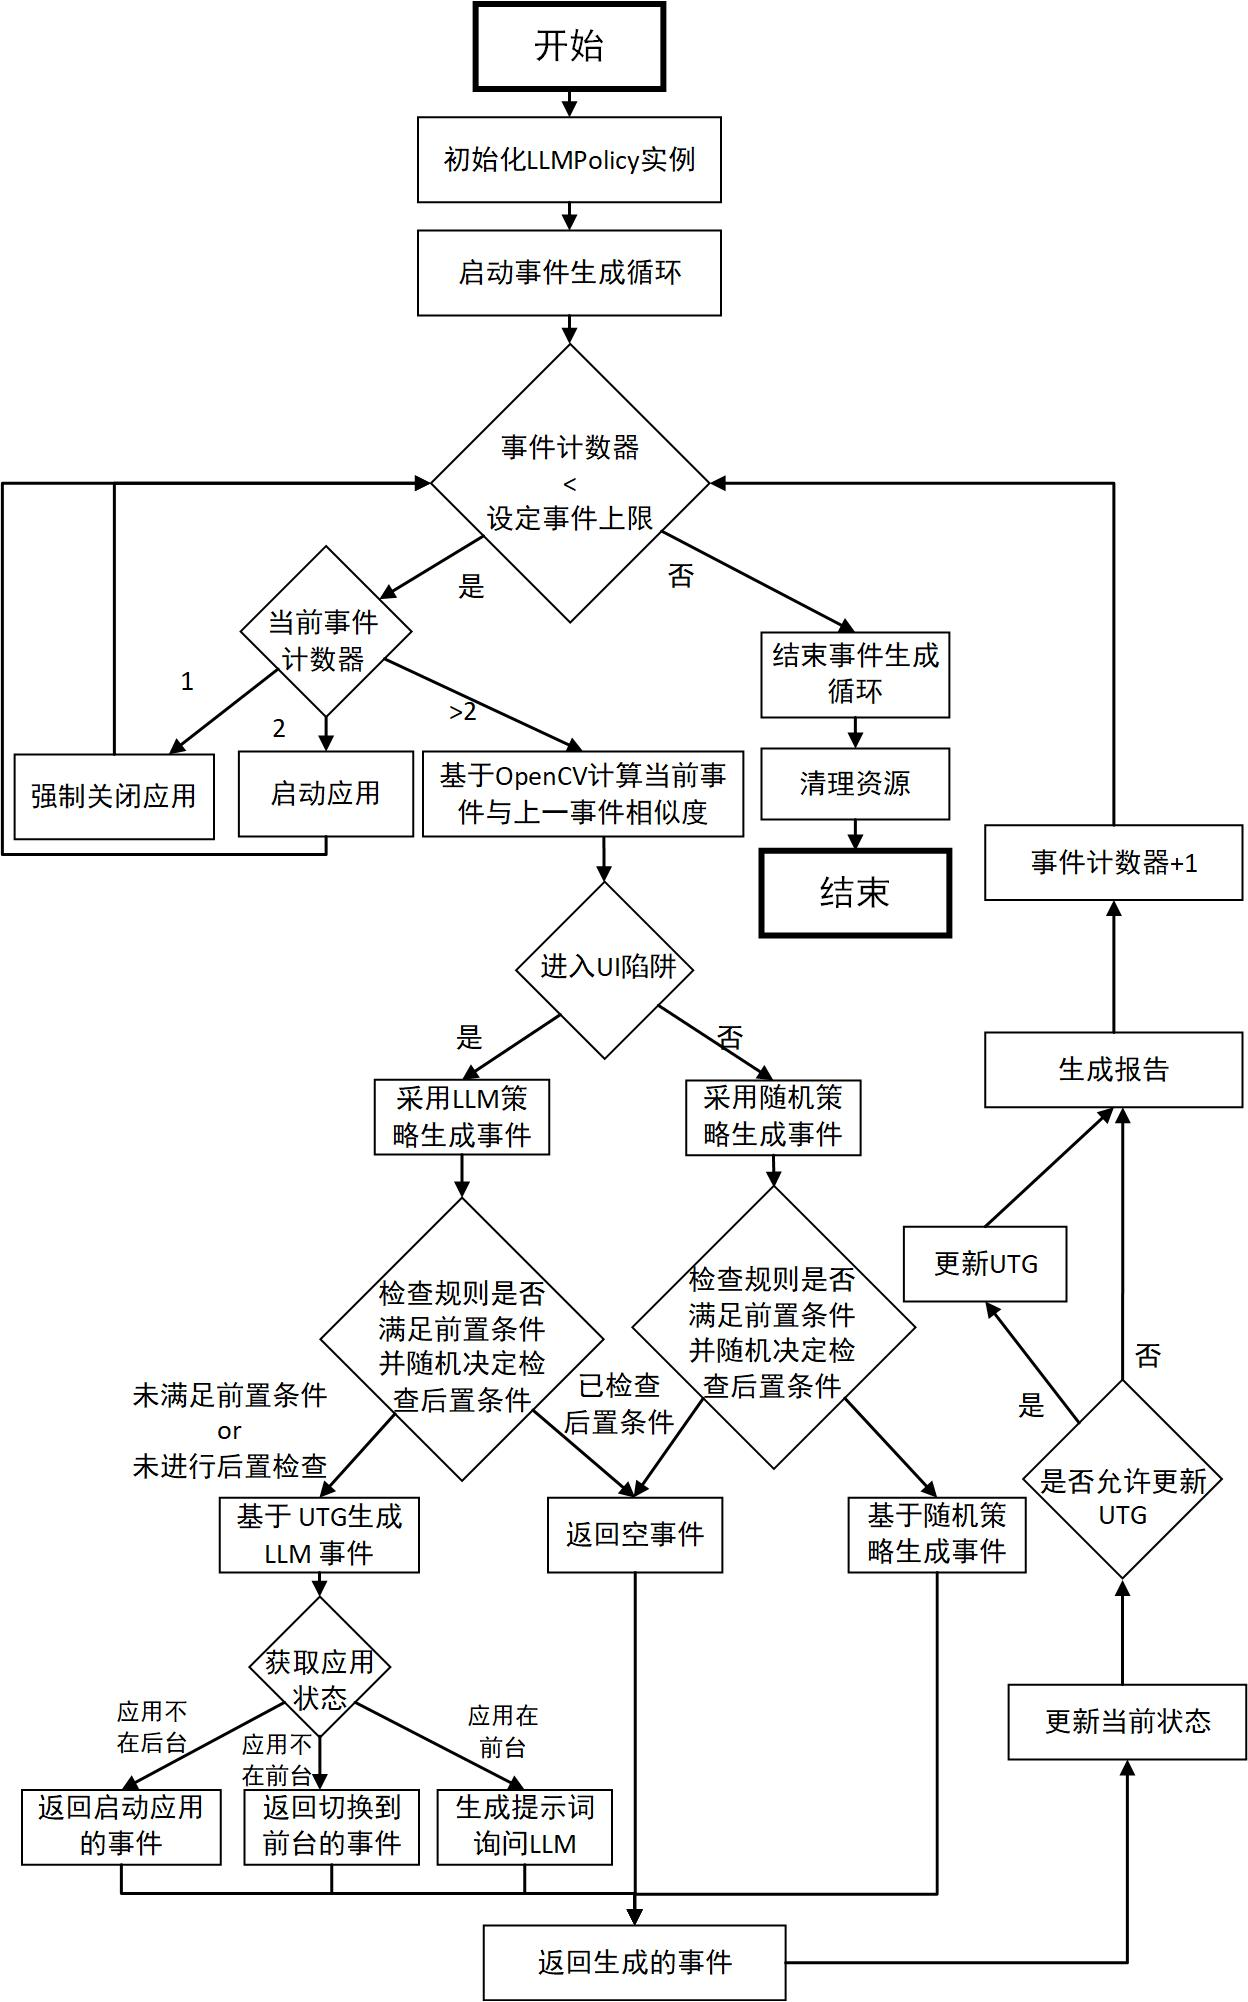
\includegraphics[width=0.8\textwidth]{software_practice_1.jpg}
    \caption{LLM 策略流程图}
    \label{fig:llm_strategy}
\end{figure}

\section*{具体步骤}

\subsection*{1. 初始化 LLMPolicy 实例}
初始化 LLMPolicy 实例,如设置日志记录器、动作历史记录等。

\subsection*{2. 启动事件生成循环}
启动事件生成循环,当生成的事件计数器大于输入管理器设定的事件计数时结束循环。

\subsubsection*{2.1 前两个事件的特殊处理}
对于前两个事件,该策略会完成初始化工作:
\begin{enumerate}[leftmargin=2em]
    \item \textbf{第一个事件:} 如果应用正在运行,\textbf{强制关闭}应用。
    \item \textbf{第二个事件:}\textbf{启动}应用。
\end{enumerate}

\subsubsection*{2.2 处理后续事件}
该策略将基于 OpenCV,获取当前应用状态的截图,并与上一个状态的截图进行比较,计算两者之间的相似度,来确定使用哪种策略生成事件。

\paragraph{2.2.1 高相似度(UI陷阱)}
满足 UI 陷阱条件(连续多次出现相似度高于阈值,次数和阈值均可通过输入管理器进行设置)时,采用 LLM 策略:
\begin{enumerate}[leftmargin=2em]
    \item 与随机生成事件策略一样,该策略会\textbf{检查规则是否满足前置条件}:
    \begin{itemize}
        \item 若满足,\textbf{随机决定}是否检查后置条件。
        \item 若进行了后置条件检查,则\textbf{不生成事件}。
    \end{itemize}
    \item 如果没有规则满足前置条件,或者策略决定不进行后置条件检查,基于 UI Transition Graph(UTG)生成 LLM 事件:
    \begin{itemize}
        \item \textbf{应用不在后台} → 返回\textbf{启动应用}的事件。
        \item \textbf{应用不在前台} → 返回\textbf{切换到前台}的事件。
        \item \textbf{应用在前台} → 生成一个提示词 Prompt。我们将当前采用的Prompt展示于后文中\ref{llm_prompt}。这一Prompt会告诉 LLM 目前的界面、交互历史,并询问下一步应该执行的操作:
        \begin{itemize}
            \item \textbf{LLM 选择操作} → 得到 LLM 回复后,返回 LLM 所选择的操作事件。如果 LLM 选择输入文本,还会再次向 LLM 询问输入的内容并返回。
            \item \textbf{LLM 选择错误或未选择} → 若 LLM 选择了错误的操作,或未选择操作,则采用随机策略生成事件。
            \item \textbf{未发现合适的交互目标} → 返回重启应用的事件。
        \end{itemize}
    \end{itemize}
\end{enumerate}

\paragraph{2.2.2 低相似度}
采用默认的\textbf{随机策略生成事件}。这一过程同样需要检查规则是否满足前置条件,以及随机检查后置条件。

\begin{tcolorbox}[colback=white, colframe=black, title=目前使用的prompt]
    \[
    \begin{aligned}
    \textbf{Task Description:} \quad
    &\text{Currently, the App is stuck on the } activity \text{ page,} \\
    &\text{unable to explore more features. Your task is to select an} \\
    &\text{action based on the current GUI information to perform} \\
    &\text{next and help the app escape the UI tarpit.}
    \end{aligned}
    \]
    
    \[
    \begin{aligned}
    \textbf{Visited Pages:} \quad
    &\text{I have already visited the following activities:}
    \end{aligned}
    \]
    
    \[
    \begin{Bmatrix}
    \text{Activity}_1 \\
    \text{Activity}_2 \\
    \vdots \\
    \text{Activity}_n
    \end{Bmatrix}
    \]
    
    \[
    \begin{aligned}
    \textbf{Failed Attempts:} \quad
    &\text{I have already completed the following steps to leave} \\
    & activity \text{ page but failed:}
    \end{aligned}
    \]
    
    \[
    \begin{Bmatrix}
    \text{Action}_1 \\
    \text{Action}_2 \\
    \vdots \\
    \text{Action}_m
    \end{Bmatrix}
    \]
    
    \[
    \begin{aligned}
    \textbf{Current State Description:} \quad &\text{State\_Prompt}
    \end{aligned}
    \]
    
    \[
    \begin{aligned}
    \textbf{Candidate Actions:} \quad &\text{Candidate\_Actions}
    \end{aligned}
    \]
    
    \[
    \begin{aligned}
    \textbf{Final Question:} \quad
    &\text{Which action should I choose next? Just return the action id} \\
    &\text{and nothing else. If no more action is needed, return -1.}
    \end{aligned}
    \]
    \label{llm_prompt}
\end{tcolorbox}

\subsubsection*{2.3 事件后续处理}
\begin{enumerate}[leftmargin=2em]
    \item 将事件添加到输入管理器,更新当前状态 \& 最后事件。
    \item 检查是否允许生成 UTG,若允许则更新 UTG。
    \item 生成报告(包括所有状态和触发的 bug 信息)。
    \item 事件计数器$+1$,回到步骤 2 继续循环。
\end{enumerate}

\subsection*{3. 结束事件生成循环}
结束事件生成循环,清理资源,结束 LLMPolicy 类的事件生成过程。

\section*{总结}

当前的大模型策略有效利用了上下文信息,使其能够更准确地理解当前App的状态和任务目标。这种策略不仅提高了LLM的决策质量,还帮助App更高效地探索新的功能。然而,我们也在探索过程中也发现了一些问题,如“几乎每一次事件的生成都由询问大模型产生”,即卡在UI陷阱频率过高。这一问题已在后续的研究中得到解决,我们将在周报中详细介绍。

\end{document}